

%%%%%%%%%%%%%%%%%%%%%%%%%%%%%%%%%%%%%%%%%12pt: grandezza carattere
                                        %a4paper: formato a4
                                        %openright: apre i capitoli a destra
                                        %twoside: serve per fare un
                                        %   documento fronteretro
                                        %report: stile tesi (oppure book)
\documentclass[12pt,a4paper,openright,twoside]{report}
%
%%%%%%%%%%%%%%%%%%%%%%%%%%%%%%%%%%%%%%%%%libreria per scrivere in italiano
\usepackage[italian]{babel}
%
%%%%%%%%%%%%%%%%%%%%%%%%%%%%%%%%%%%%%%%%%libreria per accettare i caratteri
                                        %   digitati da tastiera come � �
                                        %   si pu� usare anche
                                        %   \usepackage[T1]{fontenc}
                                        %   per� con questa libreria
                                        %   il tempo di compilazione
                                        %   aumenta
\usepackage{newlfont}

\usepackage[latin1]{inputenc}
%%\usepackage[utf8]{inputenc}

%
%%%%%%%%%%%%%%%%%%%%%%%%%%%%%%%%%%%%%%%%%libreria per impostare il documento
\usepackage{fancyhdr}
%
%%%%%%%%%%%%%%%%%%%%%%%%%%%%%%%%%%%%%%%%%libreria per avere l'indentazione
%%%%%%%%%%%%%%%%%%%%%%%%%%%%%%%%%%%%%%%%%   all'inizio dei capitoli, ...
\usepackage{indentfirst}
%%%%%%%%%%%%%%%%%%%%%%%%%%%%%%%%%%%%%%%%%libreria per inserire grafici
\usepackage{graphicx}
%
%%%%%%%%%%%%%%%%%%%%%%%%%%%%%%%%%%%%%%%%%libreria per utilizzare font
                                        %   particolari ad esempio
                                        %   \textsc{}
\graphicspath{{image/}}
\usepackage{newlfont}
%
%%%%%%%%%%%%%%%%%%%%%%%%%%%%%%%%%%%%%%%%%librerie matematiche
\usepackage{amssymb}
\usepackage{amsmath}
\usepackage{latexsym}
\usepackage{amsthm}
%\usepackage[breaklinks=true]{hyperref}
\usepackage{hyperref}
\usepackage{subfiles}
\usepackage{xcolor}
\usepackage{subfigure}
\usepackage{listings}

\definecolor{mGreen}{rgb}{0,0.6,0}
\definecolor{mGray}{rgb}{0.5,0.5,0.5}
\definecolor{mPurple}{rgb}{0.58,0,0.82}
\definecolor{backgroundColour}{rgb}{0.95,0.95,0.92}

\lstdefinestyle{CStyle}{
belowcaptionskip=1\baselineskip,
backgroundcolor=\color{backgroundColour},
  breaklines=true,
  breakatwhitespace=false,
  language=C,
  showstringspaces=false,
  basicstyle=\ttfamily\small,
  keywordstyle=\bfseries\color{green!40!black},
  commentstyle=\itshape\color{purple!40!black},
  identifierstyle=\color{blue},
  stringstyle=\color{orange}
}

\lstdefinestyle{CscriptStyle}{
belowcaptionskip=1\baselineskip,
backgroundcolor=\color{backgroundColour},
  breaklines=true,
  breakatwhitespace=false,
  language=C,
  showstringspaces=false,
  basicstyle=\ttfamily\scriptsize,
  keywordstyle=\bfseries\color{green!40!black},
  commentstyle=\itshape\color{purple!40!black},
  identifierstyle=\color{blue},
  stringstyle=\color{orange},
  tabsize=2
}


\lstdefinelanguage{Bashn}[]{bash}{
backgroundcolor=\color{backgroundColour},
commentstyle=\color{mGreen},
keywordstyle=\color{magenta},
keywordstyle=[2]\color{magenta},
numberstyle=\tiny\color{mGray},
stringstyle=\color{mPurple},
basicstyle=\ttfamily\small,
breakatwhitespace=false,
breaklines=true,
captionpos=b,
keepspaces=true,
numbers=left,
numbersep=5pt,
showspaces=false,
showstringspaces=false,
showtabs=false,
tabsize=2,
morekeywords={mkdir, git, vde_switch, vdens}
}

%
\oddsidemargin=30pt \evensidemargin=20pt%impostano i margini
\hyphenation{sil-la-ba-zio-ne pa-ren-te-si}%serve per la sillabazione: tra parentesi
					   %vanno inserite come nell'esempio le parole
%					   %che latex non riesce a tagliare nel modo giusto andando a capo.

%
%%%%%%%%%%%%%%%%%%%%%%%%%%%%%%%%%%%%%%%%%comandi per l'impostazione
                                        %   della pagina, vedi il manuale
                                        %   della libreria fancyhdr
                                        %   per ulteriori delucidazioni
\pagestyle{fancy}\addtolength{\headwidth}{20pt}
\renewcommand{\chaptermark}[1]{\markboth{\thechapter.\ #1}{}}
\renewcommand{\sectionmark}[1]{\markright{\thesection \ #1}{}}
\rhead[\fancyplain{}{\bfseries\leftmark}]{\fancyplain{}{\bfseries\thepage}}
\cfoot{}
%%%%%%%%%%%%%%%%%%%%%%%%%%%%%%%%%%%%%%%%%
\linespread{1.3}                        %comando per impostare l'interlinea
%%%%%%%%%%%%%%%%%%%%%%%%%%%%%%%%%%%%%%%%%definisce nuovi comandi
%
\begin{document}
\begin{titlepage}
\begin{center}
{{\Large{\textsc{Alma Mater Studiorum $\cdot$ Universit\`a di
Bologna}}}} \rule[0.1cm]{13.8cm}{0.1mm}
\rule[0.5cm]{13.8cm}{0.6mm}
{\bf SCUOLA DI SCIENZE\\
Corso di Laurea in Informatica }
\end{center}
\vspace{25mm}
\begin{center}
  {\large{\bf VSNLib: UN' INTERFACCIA UNICA}}\\
  \vspace{2mm}
  {\large{\bf DI CONFIGURAZIONE PER STACK VIRTUALI}}\\
  \vspace{2mm}
  {\large{\bf TRAMITE PACCHETTI NETLINK}}\\
  \end{center}
  \vspace{30mm}
  \par
  \noindent
  \begin{minipage}[t]{0.5\textwidth}
  {\large{\bf Relatore:\\
  Chiar.mo Prof.\\
  RENZO DAVOLI}}\\
  \end{minipage}
  \hfill
  \begin{minipage}[t]{0.5\textwidth}\raggedleft
  {\large{\bf Presentata da:\\
  SIMONE PREITE}}
\end{minipage}
\vspace{30mm}
\begin{center}
{\large{\bf Sessione II\\%inserire il numero della sessione in cui ci si laurea
Anno Accademico 2016/17}}%inserire l'anno accademico a cui si è iscritti
\end{center}
\end{titlepage}

%%\begin{titlepage}
\begin{center}
{{\Large{\textsc{Alma Mater Studiorum $\cdot$ Universit\`a di
Bologna}}}} \rule[0.1cm]{13.8cm}{0.1mm}
\rule[0.5cm]{13.8cm}{0.6mm}
{\bf SCUOLA DI SCIENZE\\
Corso di Laurea in Informatica }
\end{center}
\vspace{25mm}
\begin{center}
  {\large{\bf VSNLib: UN' INTERFACCIA UNICA}}\\
  \vspace{2mm}
  {\large{\bf DI CONFIGURAZIONE PER STACK VIRTUALI}}\\
  \vspace{2mm}
  {\large{\bf TRAMITE PACCHETTI NETLINK}}\\
  \end{center}
  \vspace{30mm}
  \par
  \noindent
  \begin{minipage}[t]{0.5\textwidth}
  {\large{\bf Relatore:\\
  Chiar.mo Prof.\\
  RENZO DAVOLI}}\\
  \end{minipage}
  \hfill
  \begin{minipage}[t]{0.5\textwidth}\raggedleft
  {\large{\bf Presentata da:\\
  SIMONE PREITE}}
\end{minipage}
\vspace{30mm}
\begin{center}
{\large{\bf Sessione II\\%inserire il numero della sessione in cui ci si laurea
Anno Accademico 2016/17}}%inserire l'anno accademico a cui si è iscritti
\end{center}
\end{titlepage}

\newpage
\null
\thispagestyle{empty}
\newpage

\begin{titlepage}                       %crea un ambiente libero da vincoli
                                        %   di margini e grandezza caratteri:
                                        %   si pu\`o modificare quello che si
                                        %   vuole, tanto fuori da questo
                                        %   ambiente tutto viene ristabilito
%

\thispagestyle{empty}                   %elimina il numero della pagina
\topmargin=6.5cm                        %imposta il margina superiore a 6.5cm
\raggedleft                             %incolonna la scrittura a destra
\large                                  %aumenta la grandezza del carattere
                                        %   a 14pt
\em                                     %emfatizza (corsivo) il carattere
Questa \`e la \textsc{Dedica}:\\
ognuno pu\`o scrivere quello che vuole, \\
anche nulla \ldots                      %\ldots lascia tre puntini
\end{titlepage}

\newpage
\newpage

%
%%%%%%%%%%%%%%%%%%%%%%%%%%%%%%%%%%%%%%%%
\clearpage{\pagestyle{empty}\cleardoublepage}%non numera l'ultima pagina sinistra
\pagenumbering{roman}                   %serve per mettere i numeri romani



\chapter*{Introduzione}                 %crea l'introduzione (un capitolo
                                        %   non numerato)

%%%%%%%%%%%%%%%%%%%%%%%%%%%%%%%%%%%%%%%%%imposta l'intestazione di pagina
\rhead[\fancyplain{}{\bfseries
INTRODUZIONE}]{\fancyplain{}{\bfseries\thepage}}
\lhead[\fancyplain{}{\bfseries\thepage}]{\fancyplain{}{\bfseries
INTRODUZIONE}}
%%%%%%%%%%%%%%%%%%%%%%%%%%%%%%%%%%%%%%%%%aggiunge la voce Introduzione
                                        %   nell'indice
\addcontentsline{toc}{chapter}{Introduzione}

Non vi \`e dubbio che i nodi nella rete internet siano cresciuti in maniera esponenziale fino ad oggi. Nonostante l'enorme dimensione che ha raggiunto oggi questa rete ha mantenuto gli stessi principi costruttivi che impiegava quando collegava poche macchine sperimentali: I nodi della rete sono considerati ancora le interfacce di rete degli elaboratori. Questa situazione non \`e pi\`u coerente con il funzionamento della rete internet odierna, dove il ruolo fondamentale non \`e pi\`u quello delle macchine che erogano servizi bens\`i dei servizi stessi e dei processi li forniscono.\\
La crescita smisurata dei nodi di rete e la necessit\`a di passare da un'indirizzamento di nodi all'indirizzamento di processi genera il bisogno di avere una grande quantit\`a di indirizzi per poter accedere questi processi individualmente. La famiglia di protocoli, oggi pi\`u in uso, IP vesione 4 (IPv4) risulta insufficiente per questo scopo, infatti vengono usati solamente 4 byte per indirizzare tutti i nodi accedibili direttamente.\\
Per questo gi\`a da tempo \`e in atto la migrazione verso la versione 6 del procollo IP (IPv6) che consente di avere una quantit\`a di indirizzi molto maggiore, sia per la problematica che abbiamo visto prima sia perch\'e sempre pi\`u si affacciano sulla rete dispositivi automatici capaci di agire come entit\`a autonome, oggetti provvisti di collegamenti di rete; \`e il fenomeno del cos\`i detto Internet of Things o IoT.\\
In questa ottica si colloca il presente lavoro di tesi. La realizzazione di strumenti dell'Internet of Threads (IoTh), cio\`e la possibilit\`a di assegnare indirizzi anche a singoli processi e thread, richiede l'utilizzo di stack di rete a livello del singolo processo ovvero implementati come librerie e funzionanti in spazio utente.\\
Se l'interfaccia di uso comune da parte delle applicazioni della rete ha come standard la api di Berkeley socket non esiste altrettanto standardizzata interfaccia per la configurazione e la gestione delle interfacce di rete, essendo queste, nell'ottica degli elaboratori come nodi di rete, prerogative riservate agli amministratori di sistema e non comunemente accessibili come api da parte di processi.\\
In questa tesi si studier\`a come realizzare una libreria che sia in grado di interfacciarsi ad applicazioni che usano il protocollo netlink, protocollo usato dal kernel linux per la configurazione e la gestione delle interfacce di rete, in modo da poter utilizzare, all'interno dei programmi, gli strumenti per gli amministratori di rete.\\
Nella parte seguente dell'introduzione si illustrer\`a la struttura della seguente tesi.\\
Il Prossimo capitolo presenta una rassegna dello stato dell'arte nell'ambito dei protocolli di rete e del paradigma di IoTh; nel secondo capitolo verr\`a trattato il progetto VsnLib, ovvero la libreria oggetto della tesi; infine il terzo capitolo descriver\`a alcuni esempi di utilizzo della stessa.
%%%%%%%%%%%%%%%%%%%%%%%%%%%%%%%%%%%%%%%%%non numera l'ultima pagina sinistra
\clearpage{\pagestyle{empty}\cleardoublepage}
\tableofcontents                        %crea l'indice
%%%%%%%%%%%%%%%%%%%%%%%%%%%%%%%%%%%%%%%%%imposta l'intestazione di pagina
\rhead[\fancyplain{}{\bfseries\leftmark}]{\fancyplain{}{\bfseries\thepage}}
\lhead[\fancyplain{}{\bfseries\thepage}]{\fancyplain{}{\bfseries
INDICE}}
%%%%%%%%%%%%%%%%%%%%%%%%%%%%%%%%%%%%%%%%%non numera l'ultima pagina sinistra
\clearpage{\pagestyle{empty}\cleardoublepage}
\listoffigures                          %crea l'elenco delle figure
%%%%%%%%%%%%%%%%%%%%%%%%%%%%%%%%%%%%%%%%%non numera l'ultima pagina sinistra
\clearpage{\pagestyle{empty}\cleardoublepage}
\listoftables                           %crea l'elenco delle tabelle
%%%%%%%%%%%%%%%%%%%%%%%%%%%%%%%%%%%%%%%%%non numera l'ultima pagina sinistra
\clearpage{\pagestyle{empty}\cleardoublepage}


\chapter{Internet of Threads}                %crea il capitolo
%%%%%%%%%%%%%%%%%%%%%%%%%%%%%%%%%%%%%%%%%imposta l'intestazione di pagina
\lhead[\fancyplain{}{\bfseries\thepage}]{\fancyplain{}{\bfseries\rightmark}}
\pagenumbering{arabic}                  %mette i numeri arabi
\section{Paradigma}                 %crea la sezione
IoT (Internet of Things), ovvero l'internet delle cose.\\
Questo concetto vuole rapprensentare la diffusione dei sistemi embedded come veri e propri nodi di rete, possiamo definirlo il precursore del sistema che stiamo per descrivere ed \`e il sistema che ad oggi ha permesso di incontrare il nostro condizionatore o la nostra caldaia, ma addirittura il nostro tostapane, in rete.\\
Ad un certo punto si \`e sentita l'esigenza di elevare questa astrazione, nasce il concetto di IoTh (ovvero Internet of Threads).\\
L'idea diventa quella di avere processi come nodi di rete e non oggetti fisici, l'analogia \`e molto simile alla differenza tra telefoni fissi e telefoni cellulari, ovvero in passata era necessario pensare al luogo in cui una persona potesse trovarsi,, mentre attraverso l'assegnamento di un numero personale oggi possiamo comunicare direttamente con la persona desiderata\cite{K1,K2}.\\
In termini di internet questo si traduce nella possibilit\`a di migrare servizi da un capo all'altro del mondo con la semplicit\`a di un kill and start.
Una nota va anche fatta in termini di sicurezza, ogni servizio pu\`o essere eseguito con il proprio stack di rete e questo impedirebbe a software di port mapping di carpire informazioni sulla macchina che ospita detto servizio. Inoltre possedendo il proprio stack di rete possiamo eseguire i processi con un utente non privilegiato e pertanto anche un bug del demone non comprometterebbe l'intero sistema.

\section{Stack Famosi}
Diversi sono i progetti che si occupano di offrire ai processi il proprio stack di rete; tra questi ne verranno presi in esame tre, considerati pi\`u indicati per uno studio in quanto open source.\\
Ognuno di essi offre la propria implementazione di stack di rete.
\subsection{LWIP}
Nasce da Adam Dunkels ed inizialmente non forniva supporto ad IPv6.
\subsection{LWIPv6}
\subsection{PicoTCP}
\section{Netlink}
Netlink \`e un sistema IPC (Inter Process Comunication) usato perch\`e in grado di mettere in comunicazione diversi task, solitamente serve per far comunicare task in user-space con task in kernel-space ma pu\`o far interagire anche processi entrambi in user-space.\\
Studiato per essere il successore di ioctl per le configurazioni ed il monitoraggio, si propone di essere pi\`u flessibile
\subsection{Inter Process Comunication}
Molti processi necessitano di scambiare informazioni per i motivi pi\`u disparati, dalla comunicazion e di rete a quella interna ad una sola macchina.\\
Viene da se pensare che costruire programmi che non interagiscono con il mondo esterno o con altri programmi sarebbe una risorsa limitata.\\
Con IPC intendiamo quindi l'insieme delle tecnologie adottate per permettere ai processi di comunicare tra essi, che siano ospitati sulla stessa macchina o distribuiti sulla rete, tra queste tecnologie esiste appunto quella utilizzata all'interno della libreria oggetto di questo elaborato.
\subsection{Libnl}
Netlink Protocol Library Suite (libnl), \`e una raccolta di librerie ed utility che forniscono API di comunicazione netlink basate su quelle del kernel linux e comprende \cite{K10}:
\begin{description}                     %crea un elenco descrittivo
  \item[libnl] Core della libreria, offre uno strato di unificazione delle interfacce sulle quali poi si basano le altre librerie che pertanto di pendo da questa;
  \item[libnl-route] Questa libreria si occupa di fornire API per la configurazione degli elemnti della famiglia NETLINK\_ROUTE;
  \item[libnl-genl] genl significa generic netlink e questa libreria offre una versione estesa del protocollo netlink;
  \item[libnl-nf] API per configurazioni netlink basate su netfilter.

\end{description}
%%%%%%%%%%%%%%%%%%%%%%%%%%%%%%%%%%%%%%%%%non numera l'ultima pagina sinistra

\clearpage{\pagestyle{empty}\cleardoublepage} 



\chapter{VSNLib}                %crea il capitolo
%%%%%%%%%%%%%%%%%%%%%%%%%%%%%%%%%%%%%%%%%imposta l'intestazione di pagina
\lhead[\fancyplain{}{\bfseries\thepage}]{\fancyplain{}{\bfseries\rightmark}}
Interfaccia di configurazione degli stack di rete attraverso l'utilizzo di tecnologia netlink.
\section{Il Progetto}                 %crea la sezione
Gli stack analizzati in precedenza offrono a grandi linee la stessa tipologia di servizio seppur ognuna con le proprie caratteristice.\\
Nessuno dei progetti ha per\`o tenuto in considerazione l'idea di utilizzare un'interfaccia di configurazione che fosse standard, \`e pertanto necessario usare le funzioni specifiche per ognuno di questi progetti, costringendo il programmatore a cambiare modalit\`a di interazione da stack a stack.\\
L'idea di creare questa libreria nasce proprio dall' esigenza di uniformare le interfacce di comunicazione in modo tale che l'utente non sia costretto ad adattarsi ogni qual volta decida di cambiare stack.\\
\section{VSNLib}
\subsection{Preambolo}
Per configurare uno stack di rete programmi come ip generano un pacchetto netlink con le informazioni necessarie lo inviano al kernel che lo elabora, esegue le operazioni e genera un messaggio contenente un flag attraverso il quale viene comunicato il tipo di errore (0 in caso di successo). A questo messaggio \`e associato un payload di risposta generalmente usato per comporre un feedback da mostrare all'utente che sta interagendo con il programma, in figura \ref{fig:nlmserror} lo schema dell'header per il messaggio di risposta.\\
\begin{figure}[h]                       %crea l'ambiente figura; [h] sta
                                        %   per here, cio� la figura va qui
\begin{center}                          %centra nel mezzo della pagina
                                        %   la figura
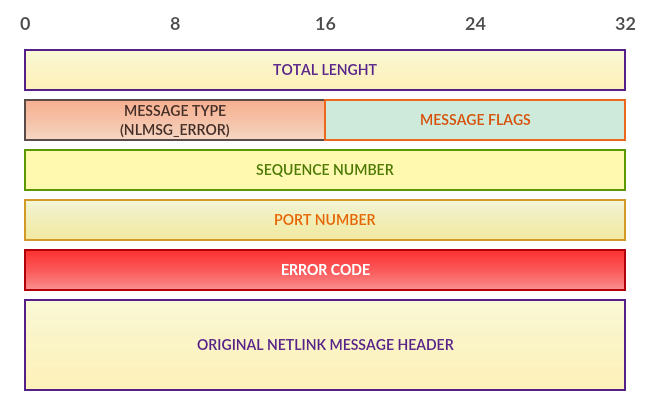
\includegraphics[width=10cm]{nlmsgerror}%inserisce una figura larga 5cm
                                        %se si vuole usare va scommentata
%
%%%%%%%%%%%%%%%%%%%%%%%%%%%%%%%%%%%%%%%%%inserisce la legenda ed etichetta
                                        %   la figura con \label{fig:prima}
\caption[struct nlmserror]{schema della struttura per il messaggio di risposta}\label{fig:nlmserror}
\end{center}
\end{figure}
VSNLib \`e un progetto in fase di sviluppo scritto in C e completamente opensource, liberamente scaricabile attraverso la piattaforma github al seguente link \url{https://github.com/simonepreite/vsnlib}.

\subsection{Ambiente}
La necessit\`a primaria: catturare queste comunicazioni netlink.\\
Per farlo si \`e reso necessario intercettare la system call di invio della richiesta contenente il payload; ovvero l'esecuzione della sendto, verso il socket netlink sotto la nostra attenzione, contenente il buffer della richiesta.\\
In questo punto interviene la nostra libreria, che si interpone e di fatto fa le veci del kernel, al quale il pacchetto netlink non arriver\`a mai realmente.\\
In partenza VSNLib utilizzava come motore di cattura delle system call la libreria purelibc\cite{K8}, in seguito per\`o si \`e giunti alla conclusione che costruire un modulo ad hoc all'interno del sistema vuos fosse un'alternativa pi\`u versatile, immediata e pulita, inoltre vuos ha un sistema di debug built in che rende pi\`u semplice l'individuazione dei problemi legati allo sviluppo.\\
Vuos\cite{K5} \`e un progetto di virtualsquare, ha come obiettivo quello di virtualizzare parti del sistema operativo senza negare all'utilizzatore la scelta degli elementi da virtualizzare, \`e costruito con un sistema di moduli che possono essere aggiunti a discrezione dell'utente.\\
La versione di sviluppo ufficiale \`e liberamente scaricabile attraverso la piattaforma github al seguente link \url{https://github.com/virtualsquare/vuos}. \\
Per il testing \`e stato creato un fork di vuos contenente il modulo relativo alla cattura delle system call di interesse per VSNLib, anche questa versione reperibile risiede su github \url{https://github.com/simonepreite/vuos}.\\
Il modulo in questione si chiama unrealvsnlib per analogia alla libreria ma ognuno \`e libero di costruire un proprio modulo che si adatti alle esigenze di sviluppo personali.\\

\subsection{Schema}
La libreria costituisce uno strato  intermedio di compatibilit\`a tra netlink e le specifiche configurazioni degli stack.\\
Vediamo come \`e composta:
\begin{description}                     %crea un elenco descrittivo
  \item[VSNLib:] Il primo strato si occupa di inizializzare la libreria in base allo stack che si intende utilizzare (informazione richiesta all'utente) e di mediare la comunicazione tra netlink ed il modulo scelto.\\
  Indicare esplicitamente il modulo desiderato \`e una scelta implementativa dettata dal principio di avere un core che sia il pi\`u contenuto possibile.
  \item[Modules:] Sono la parte specifica della libreria, essi contengono l'intestazione delle funzioni generiche che si occupano di chiamare quelle particolari per ogni stack.
\end{description}
\begin{figure}[h]                       %crea l'ambiente figura; [h] sta
                                        %   per here, cio� la figura va qui
\begin{center}                          %centra nel mezzo della pagina
                                        %   la figura
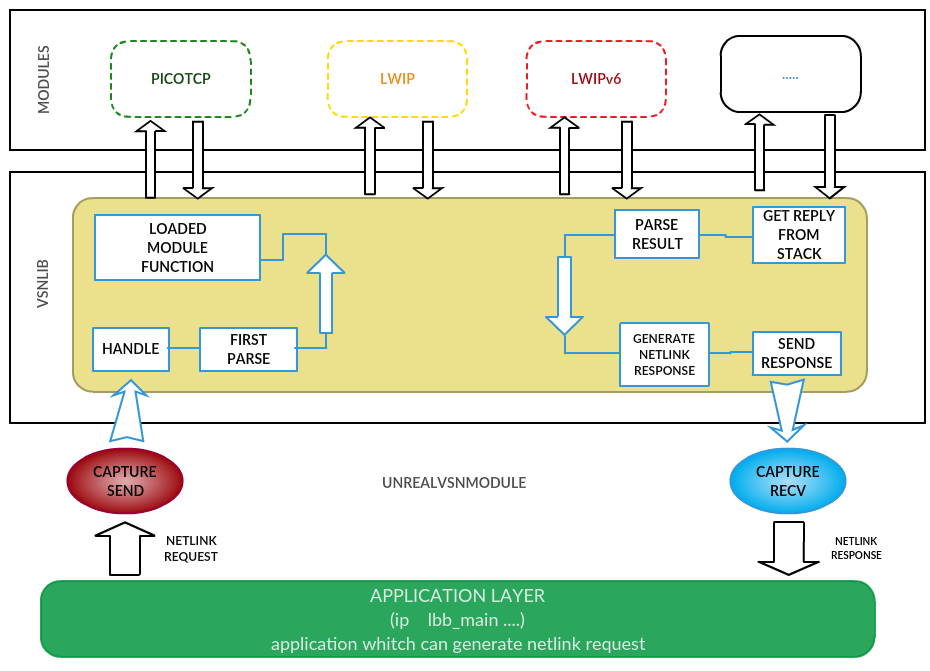
\includegraphics[width=14cm]{vsnlib_scheme}%inserisce una figura larga 5cm
                                        %se si vuole usare va scommentata
%
%%%%%%%%%%%%%%%%%%%%%%%%%%%%%%%%%%%%%%%%%inserisce la legenda ed etichetta
                                        %   la figura con \label{fig:prima}
\caption[mappa concettuale libreria]{mappa concettuale libreria}\label{fig:map}
\end{center}
\end{figure}
\subsection{VSNLib}
Espone le interfacce di comunicazione della libreria, che di fatto sono due, una per inizializzare l'ambiente ed una per inviare il pacchetto da gestire.\\
\begin{lstlisting}[style=CStyle]
int init_vsnlib(char* stack);
void handle_vsnlib(void* buf, size_t len, void* nif, void* stack);
\end{lstlisting}
La prima funzione \`e di inizializzazione della libreria e tramite dlopen ed il nome del modulo da caricare si incarica di popolare l'array di puntatori con i corrispettivi delle funzioni nel modulo.\\
La seconda funzione contiene un loop che cicla sui messaggi del paccheto netlink, che di fatto potrebbero essere pi\`u di uno. Per ogni messaggio ne viene analizzata la tipologia ed in base al tipo si accede all'emento dell'array che contiene il puntatore alla funzione adeguata a svolgere quel compito.\\
L'utente non ha accesso ad altre funzioni perch\'e \`e la libreria stessa ad analizzare il pacchetto, riempire i campi della struttura generica ed inviarlo al modulo relspecifico dello stack.\\
In risposta si ricever\`a una struttura adatta alla costruzione del paccehetto netlink da spedire alla system call recvfrom del programma in attesa, questo \`e l'ultimo compito della nostra libreria.
\subsection{Moduli}
La presenza di moduli per gestire i vari stack lascia la libert\`a a chiunque necessiti di uno stack non supportato, o personalizzato, di creare il proprio modulo rispettando le specifiche della libreria.\\
Ogni modulo, infatti, ha la stessa struttura e contiene azioni generiche comuni in tutti gli stack. Possiamo vedere i prototipi di una di queste funzioni qui di seguito.
\begin{lstlisting}[style=CStyle]
struct response* adddeladdr(struct config* cfg);
struct response* getaddr(struct config* cfg);
struct response* adddellink(struct config* cfg);
struct response* getsetlink(struct config* cfg);
struct response* adddelroute(struct config* cfg);
struct response* getroute(struct config* cfg);
\end{lstlisting}
In breve ogni modulo \`e composto dallo stesso numero di funzioni che si occupano di mediare la comunicazione tra la libreria e il vero stack.
Ognuna di queste ha un'implementazione diversa a seconda del modulo.\\
Grazie alla tecnica dei puntatori a funzione, si riesce ad essere abbastanza generali e possiamo evitare di specificarne il nome completo.\\
L'idea \`e stata quella di inizializzare, in fase di caricamento della libreria (che avviene con dlopen), un array di puntatori a funzione (attraverso dlsym) in modo tale da poter effettuare le chiamate attraverso di esso. Dlopen e dlsym permettono di caricare dinamicamente solo il modulo di cui si necessita.\\
All' interno dei moduli le funzioni ricevono in input lo stesso tipo di struttura. Durante l'esecuzione di un'azione loro compito \`e la raccola di informazioni dalle funzioni reali dello stack che verranno poi usate per riempire i campi della struttura di risposta che a sua volta servir\`a a creare il payload per il pacchetto netlink di risposta.
%%%%%%%%%%%%%%%%%%%%%%%%%%%%%%%%%%%%%%%%%non numera l'ultima pagina sinistra
\clearpage{\pagestyle{empty}\cleardoublepage}



\chapter{Casi d'uso}                %crea il capitolo
%%%%%%%%%%%%%%%%%%%%%%%%%%%%%%%%%%%%%%%%%imposta l'intestazione di pagina
\lhead[\fancyplain{}{\bfseries\thepage}]{\fancyplain{}{\bfseries\rightmark}}
Di seguito alcuni esempi di utilizzo della libreria.
Le dimostrazioni seguenti sono state effettuate su una macchina con architettura amd64 e con installato il sistema operativo debian in versione sid (quindi unstable) ma sono state testate e riprodotteanche su altre configurazioni e distribuzioni GNU/Linux.

\section{Esempi}                 %crea la sezione

%%%%%%%%%%%%%%%%%%%%%%%%%%%%%%%%%%%%%%%%%non numera l'ultima pagina sinistra
\clearpage{\pagestyle{empty}\cleardoublepage} 



%%%%%%%%%%%%%%%%%%%%%%%%%%%%%%%%%%%%%%%%%per fare le conclusioni
\chapter*{Conclusioni}
%%%%%%%%%%%%%%%%%%%%%%%%%%%%%%%%%%%%%%%%%imposta l'intestazione di pagina
\rhead[\fancyplain{}{\bfseries
CONCLUSIONI}]{\fancyplain{}{\bfseries\thepage}}
\lhead[\fancyplain{}{\bfseries\thepage}]{\fancyplain{}{\bfseries
CONCLUSIONI}}
%%%%%%%%%%%%%%%%%%%%%%%%%%%%%%%%%%%%%%%%%aggiunge la voce Conclusioni
                                        %   nell'indice
\addcontentsline{toc}{chapter}{Conclusioni}
L'utilizzo di queste tipologie di stack dipende strettamente dalla diffusione del protocollo IPv6 e dei sistemi embedded.
La ricerca e lo sviluppo di questi meccanismi sono necessari ad ottenere un sistema performante e stabile quando IPv6 sar\`a l'ordinario. Vanno inoltre considerati i vantaggi conseguenti nelle reti virtuali che gi\`a ora vengono utilizzate per la sperimentazione e che in futuro saranno sicuramente di larga diffusione.\\
L'indipendenza dalle infrastrutture fisiche \`e un vantaggio non indifferente, significa che le reti ed i sistemi possono essere creati, modificati o ricostruiti da zero con estrema facilit\`a. Basti pensare ad una rete di macchine virtuali, trattandosi di software pu\`o essere ampliata con nuovi elaboratori virtuali, spenta e modificata senza dover invesitire in nuovo hardware.\\
Quelli esposti sono solo alcuni dei vantaggi sufficienti a lasciare intendere la direzione verso cui questo settore sta proseguendo.


\chapter*{Sviluppi Futuri}
%%%%%%%%%%%%%%%%%%%%%%%%%%%%%%%%%%%%%%%%%imposta l'intestazione di pagina
\rhead[\fancyplain{}{\bfseries
Sviluppi Futuri}]{\fancyplain{}{\bfseries\thepage}}
\lhead[\fancyplain{}{\bfseries\thepage}]{\fancyplain{}{\bfseries
SVILUPPI FUTURI}}
%%%%%%%%%%%%%%%%%%%%%%%%%%%%%%%%%%%%%%%%%aggiunge la voce Conclusioni
                                        %   nell'indice
\addcontentsline{toc}{chapter}{Sviluppi Futuri}
In fase di progettazione non sono stati posti limiti alla crescita del progetto e la sua modularit\`a \`e legata principalmente a questo aspetto.\\
L'augurio \`e che questo progetto continui a crescere arricchendosi di funzionalit\`a.\\
In questa fase ci si \`e occupati delle configurazioni e del routing che deve essere completata e testata prima di poter affermarne la stabilit\`a.\\
Senz'altro aumentare il supporto agli stack meno conosciuti ed a quelli che in futuro saranno sviluppati \`e il prosieguo pi\`u ovvio per VSNLib.
Tra le altre ipotesi di ampliamento c'\`e quella di gestione del filtering, l'intento in questo caso sar\`a fornire un'interfaccia identica a quella di iptables ma per settare le regole di filtraggio sugli stack virtuali.\\


%%%%%%%%%%%%%%%%%%%%%%%%%%%%%%%%%%%%%%%%%imposta l'intestazione di pagina
\renewcommand{\chaptermark}[1]{\markright{\thechapter \ #1}{}}
\lhead[\fancyplain{}{\bfseries\thepage}]{\fancyplain{}{\bfseries\rightmark}}
\appendix                               %imposta le appendici
\chapter{Core}               %crea l'appendice
\label{code:AppA}
%%%%%%%%%%%%%%%%%%%%%%%%%%%%%%%%%%%%%%%%%imposta l'intestazione di pagina
\rhead[\fancyplain{}{\bfseries \thechapter \:Core}]
{\fancyplain{}{\bfseries\thepage}}
vsnshared.h
\begin{lstlisting}[style=CscriptStyle]
#ifndef _VSNSHARED_H
#define _VSNSHARED_H

#include <asm/types.h>
#include <linux/netlink.h>
#include <linux/rtnetlink.h>
#include <arpa/inet.h>

struct response{
	int error; //0 for success
};

extern void handle_vsnlib(void* buf, size_t len, void* nif, void* stack);
extern int init_vsnlib(char* stack);

#endif

\end{lstlisting}
vsnlib.h
\begin{lstlisting}[style=CscriptStyle]
#ifndef _VSNLIB_H
#define _VSNLIB_H

#include "vsnshared.h"

#define  API_TABLE_SIZE 6

/* struct definition */
struct config{
	char* addr;
	int mask;
	int family;
	void* interface;
	void* stack; // stack file descriptor
	int operation;
};

typedef struct response* (*generic_api)(struct config* cfg);
struct gen_api{
  char* fun_name;
  generic_api real_fun;
};

static struct gen_api api_table[]={
  {"adddellink", NULL},
  {"getsetlink",NULL},
  {"adddeladdr", NULL},
  {"getaddr", NULL},
  {"adddelroute", NULL},
  {"getroute", NULL}
};

/* client side */

struct nlmsghdr* rtm_newroute_c(struct nlmsghdr* header, void* nif, void* stack);
struct nlmsghdr* rtm_delroute_c(struct nlmsghdr* header, void* nif, void* stack);
struct nlmsghdr* rtm_getroute_c(struct nlmsghdr* header, void* nif, void* stack);
struct nlmsghdr* rtm_newaddr_c(struct nlmsghdr* header, void* nif, void* stack);
struct nlmsghdr* rtm_deladdr_c(struct nlmsghdr* header, void* nif, void* stack);
struct nlmsghdr* rtm_getaddr_c(struct nlmsghdr* header, void* nif, void* stack);
struct nlmsghdr* rtm_newlink_c(struct nlmsghdr* header, void* nif, void* stack);
struct nlmsghdr* rtm_dellink_c(struct nlmsghdr* header, void* nif, void* stack);
struct nlmsghdr* rtm_getlink_c(struct nlmsghdr* header, void* nif, void* stack);
struct nlmsghdr* rtm_setlink_c(struct nlmsghdr* header, void* nif, void* stack);

typedef struct nlmsghdr* vsn_cli(struct nlmsghdr* header, void* nif, void* stack);
static vsn_cli *vsncli_fun_table[]={
	/* NEW/DEL/GET/SET link */
  rtm_newlink_c,
  rtm_dellink_c,
  rtm_getlink_c,
  rtm_setlink_c,
	/* NEW/DEL/GET addr */
  rtm_newaddr_c,
  rtm_deladdr_c,
  rtm_getaddr_c,
  NULL,
	/* NEW/DEL/GET route */
  rtm_newroute_c,
  rtm_delroute_c,
  rtm_getroute_c,
  NULL
};

#endif

\end{lstlisting}

vsnlib.c
\begin{lstlisting}[style=CscriptStyle]
#include <stdio.h>
#include <stdlib.h>
#include <fcntl.h>
#include <unistd.h>
#include <dirent.h>
#include <string.h>
#include <dlfcn.h>

#include <vsnlib.h>
#include <vsnshared.h>


struct ret_val{
  struct nlmsghdr* res;
  struct ret_val* next;
};

char* combine_stack_handler(char* fun_name, char* stack){
    //rimuove il .so
    char* combo;
    int len_stack = strlen(stack)-1;
    combo = malloc(sizeof(char)*(strlen(fun_name)+(len_stack-1)));
    strcpy(combo, stack);
    combo[len_stack-2] = '_';
    combo[len_stack-1] = '\0';
    strcat(combo, fun_name);
    return combo;
}


int init_vsnlib(char* stack){
  const char *error;
  char* f;
  void *stack_module;

  stack_module = dlopen(stack,RTLD_LAZY);
  if(!stack_module){
    fprintf(stderr, "Cannot open stack library: %s\n",
    dlerror());
    return -1;
  }
  for(int i=0; i < API_TABLE_SIZE; i++){
    api_table[i].real_fun = dlsym(stack_module, api_table[i].fun_name);
    if ((error = dlerror())) {
      fprintf(stderr, "Couldn't find %s: %s\n", api_table[i].fun_name, error);
      exit(1);
    }
  }
  return 0; //if success
}

void handle_vsnlib(void* buf, size_t len, void* nif, void* stack){
  struct nlmsghdr* header = (struct nlmsghdr*) buf;
  struct nlmsghdr* ret_pkg;
  while (NLMSG_OK(header, len)) {
    /*int err;*/
    int type;

    if (header->nlmsg_type == NLMSG_DONE)
      break;
    type=header->nlmsg_type - RTM_BASE;
    header->nlmsg_pid=getpid();
    if (type >= 0 && vsncli_fun_table[type] != NULL) {
        struct ret_val* app = malloc(sizeof(struct ret_val));
        (vsncli_fun_table[type](header, nif, stack));
    }
    header = NLMSG_NEXT(header, len);
  }
}

struct nlmsghdr* rtm_newlink_c(struct nlmsghdr* header, void* nif, void* stack){
  struct ifinfomsg* ifi = (struct ifinfomsg*)(NLMSG_DATA(header));
  struct config generic_conf;
  struct response* generic_resp;
  generic_conf.interface = nif;
  generic_conf.operation = ifi->ifi_flags;
  generic_resp = api_table[0].real_fun(&generic_conf);
}

struct nlmsghdr* rtm_dellink_c(struct nlmsghdr* header, void* nif, void* stack){
  struct ifinfomsg* ifi = (struct ifinfomsg*)(NLMSG_DATA(header));
  struct config* generic_conf;
  struct response* generic_resp;
  generic_resp = api_table[0].real_fun(generic_conf);
}

struct nlmsghdr* rtm_getlink_c(struct nlmsghdr* header, void* nif, void* stack){
  struct ifinfomsg* ifi = (struct ifinfomsg*)(NLMSG_DATA(header));
  struct config* generic_conf;
  struct response* generic_resp;
  generic_resp = api_table[1].real_fun(generic_conf);
}

struct nlmsghdr* rtm_setlink_c(struct nlmsghdr* header, void* nif, void* stack){
  struct ifinfomsg* ifi = (struct ifinfomsg*)(NLMSG_DATA(header));
  struct config* generic_conf;
  struct response* generic_resp;
  generic_resp = api_table[1].real_fun(generic_conf);
}

struct nlmsghdr* rtm_newaddr_c(struct nlmsghdr* header, void* nif, void* stack){
  struct ifaddrmsg* ifa = (struct ifaddrmsg*)(NLMSG_DATA(header));
  struct config generic_conf;
  struct response* generic_resp;
  char str6[INET6_ADDRSTRLEN];
  char* str4;
  generic_conf.operation=header->nlmsg_type;
  generic_conf.interface=nif;
  generic_conf.mask=ifa->ifa_prefixlen;
  generic_conf.family=ifa->ifa_family;
  struct rtattr* attr = (struct rtattr*)((void*)(((char*)ifa)+ sizeof(struct ifaddrmsg)));
  if(ifa->ifa_family == AF_INET6){
    struct in6_addr* ip6_a = (struct in6_addr*)RTA_DATA(attr);
    inet_ntop(ifa->ifa_family, ip6_a, str6, INET6_ADDRSTRLEN);
    inet_pton(ifa->ifa_family, str6, ip6_a);
    generic_conf.addr=str6;
  }
  else{
    struct in_addr ip4_a = *((struct in_addr*)RTA_DATA(attr));
    str4 = inet_ntoa(ip4_a);
    generic_conf.addr=str4;
  }
  generic_conf.stack=stack;
  generic_resp = api_table[2].real_fun(&generic_conf);
}

struct nlmsghdr* rtm_deladdr_c(struct nlmsghdr* header, void* nif, void* stack){
  rtm_newaddr_c(header, nif, stack);
}

struct nlmsghdr* rtm_getaddr_c(struct nlmsghdr* header, void* nif, void* stack){
  struct ifaddrmsg* ifa = (struct ifaddrmsg*)(NLMSG_DATA(header));
  struct config* generic_conf;
  struct response* generic_resp;
  generic_resp = api_table[3].real_fun(generic_conf);
}

struct nlmsghdr* rtm_newroute_c(struct nlmsghdr* header, void* nif, void* stack){
  struct rtmsg* rtm = (struct rtmsg*)(NLMSG_DATA(header));
  struct config generic_conf;
  struct response* generic_resp;
  char str6[INET6_ADDRSTRLEN];
  char* str4;

  generic_conf.operation=header->nlmsg_type;
  generic_conf.interface=nif;
  generic_conf.family=rtm->rtm_family;
  generic_conf.stack=stack;
  struct rtattr* attr = (struct rtattr*)((void*)(((char*)rtm)+ sizeof(struct rtmsg)));
  if(rtm->rtm_family == AF_INET6){
    struct in6_addr* ip6_a = (struct in6_addr*)RTA_DATA(attr);
    inet_ntop(rtm->rtm_family, ip6_a, str6, INET6_ADDRSTRLEN);
    generic_conf.addr=str6;
  else{
    struct in_addr ip4_a = *((struct in_addr*)RTA_DATA(attr));
    str4 = inet_ntoa(ip4_a);
    generic_conf.addr=str4;
  }
  generic_resp = api_table[4].real_fun(&generic_conf);
  }
}

struct nlmsghdr* rtm_delroute_c(struct nlmsghdr* header, void* nif, void* stack){
  rtm_newroute_c(header, nif, stack);
}

struct nlmsghdr* rtm_getroute_c(struct nlmsghdr* header, void* nif, void* stack){
  struct rtmsg* rtm = (struct rtmsg*)(NLMSG_DATA(header));
  struct config* generic_conf;
  struct response* generic_resp;
  generic_resp = api_table[5].real_fun(generic_conf);
}

\end{lstlisting}

\chapter{Modules}               %crea l'appendice
\label{code:AppB}
%%%%%%%%%%%%%%%%%%%%%%%%%%%%%%%%%%%%%%%%%imposta l'intestazione di pagina
\rhead[\fancyplain{}{\bfseries \thechapter \:Modules}]
{\fancyplain{}{\bfseries\thepage}}
vsnmodules.h
\begin{lstlisting}[style=CscriptStyle]

\end{lstlisting}

LWIPv6.c
\begin{lstlisting}[style=CscriptStyle]
#include <stdio.h>
#include <vsnlib.h>
#include <lwipv6.h>


struct response* adddeladdr(struct config* cfg){
  struct ip_addr addr;
  struct ip_addr mask;
  uint16_t* p_mask = NULL;

  if(cfg->family == AF_INET6){
    uint16_t mask_app[8]={0,0,0,0,0,0,0,0};
    struct in6_addr ip6;

    uint16_t* p = (uint16_t*)(&ip6);
    p_mask = (uint16_t*)(&mask_app);

    for(int i=0; i<8; i++){
      *p=0;
      p++;
    }
    p = (uint16_t*)(&ip6);
    inet_pton(cfg->family, cfg->addr, &ip6);

    while(cfg->mask > 0){
      *p_mask = 0xffff;
      cfg->mask-= 16;
      p_mask++;
    }

    p_mask = (uint16_t*)(&mask_app);

    printf("ipv6 addr: %04X::%04X::%04X::%04X::%04X::%04X::%04X::%04X\n",htons(*(p)),htons(*(p+1)),htons(*(p+2)),htons(*(p+3)),htons(*(p+4)),htons(*(p+5)),htons(*(p+6))htons(*(p+7)));
    IP6_ADDR(&addr,htons(*(p)),htons(*(p+1)),htons(*(p+2)),htons(*(p+3)),htons(*(p+4)),htons(*(p+5)),htons(*(p+6)),htons(*(p+7)));
    printf("mask: %04X::%04X::%04X::%04X::%04X::%04X::%04X::%04X\n",*(p_mask),*(p_mask+1),*(p_mask+2),*(p_mask+3),*(p_mask+4),*(p_mask+5),*(p_mask+6),*(p_mask+7));
    IP6_ADDR(&mask,*(p_mask),*(p_mask+1),*(p_mask+2),*(p_mask+3),*(p_mask+4),*(p_mask+5),*(p_mask+6),*(p_mask+7));
  }
  else{
    struct in_addr ip4;
    uint16_t lwip_mask4[4] = {0,0,0,0};
    p_mask = (uint16_t*)(&lwip_mask4);
    while(cfg->mask > 0){
      *p_mask=255;
      cfg->mask -= 8;
      p_mask++;
    }
    inet_aton(cfg->addr, &ip4);
    unsigned char ip4_dot[4];
    int j=0;
    for(int i=0; i<4; i++){
      ip4_dot[i]=(ip4.s_addr >> j) & 0xFF;
      j=j+8;
    }
    printf("ipv4 address: %d.%d.%d.%d\n",ip4_dot[0],ip4_dot[1],ip4_dot[2],ip4_dot[3]);
    IP64_ADDR(&addr,ip4_dot[0],ip4_dot[1],ip4_dot[2],ip4_dot[3]);
    printf("ipv4 mask: %d.%d.%d.%d\n",lwip_mask4[0],lwip_mask4[1],lwip_mask4[2],lwip_mask4[3]);
    IP64_MASKADDR(&mask,lwip_mask4[0],lwip_mask4[1],lwip_mask4[2],lwip_mask4[3]);
  }
  if(cfg->operation == RTM_NEWADDR){
    printf("error add addr lwipv6: %d\n", lwip_add_addr((struct netif*)(cfg->interface),&addr,&mask));
  }
  else if (cfg->operation == RTM_DELADDR) {
    printf("error del addr lwipv6: %d\n", lwip_del_addr((struct netif*)(cfg->interface),&addr,&mask));
  }
}

struct response* getaddr(struct config* cfg){

}

struct response* adddellink(struct config* cfg){
  printf("adddellink\n");
  if(cfg->operation == 1)
    printf("ifup: %d\n", lwip_ifup((struct netif*)(cfg->interface)));
  else
    printf("ifdown: %d\n", lwip_ifdown((struct netif*)(cfg->interface)));
}

struct response* getsetlink(struct config* cfg){

}

struct response* adddelroute(struct config* cfg){
  struct ip_addr addr;

  if(cfg->family==AF_INET6){
    struct in6_addr address;
    uint16_t* p = (uint16_t*)(&address);
    p = (uint16_t*)(&address);
    inet_pton(cfg->family, cfg->addr, &address);
    printf("ipv6 addr: %04X::%04X::%04X::%04X::%04X::%04X::%04X::%04X\n",htons(*(p)),htons(*(p+1)),htons(*(p+2)),htons(*(p+3)),htons(*(p+4)),htons(*(p+5)),htons(*(p+6))htons(*(p+7)));
    IP6_ADDR(&addr,htons(*(p)),htons(*(p+1)),htons(*(p+2)),htons(*(p+3)),htons(*(p+4)),htons(*(p+5)),htons(*(p+6)),htons(*(p+7)));
  }
  else{
    struct in_addr ip4;
    inet_aton(cfg->addr, &ip4);
    unsigned char ip4_dot[4];
    int j=0;
    for(int i=0; i<4; i++){
      ip4_dot[i]=(ip4.s_addr >> j) & 0xFF;
      j=j+8;
    }
    printf("ipv4 route: %d.%d.%d.%d\n",ip4_dot[0],ip4_dot[1],ip4_dot[2],ip4_dot[3] );
    IP64_ADDR(&addr,ip4_dot[0],ip4_dot[1],ip4_dot[2],ip4_dot[3]);
  }

  if(cfg->operation==RTM_NEWROUTE){
    printf("error add route lwipv6 %d\n", lwip_add_route((struct stack*)cfg->stack, IP_ADDR_ANY, IP_ADDR_ANY, &addr, (struct netif*)(cfg->interface),0));
  }
  else if(cfg->operation==RTM_DELROUTE){
    printf("error del route lwipv6: %d\n", lwip_del_route((struct stack*)cfg->stack, IP_ADDR_ANY, IP_ADDR_ANY, &addr, (structnetif*)(cfg->interface), 0));
  }
}

struct response* getroute(struct config* cfg){

}

\end{lstlisting}

\chapter{Test}             %crea l'appendice
\label{code:AppC}
\rhead[\fancyplain{}{\bfseries \thechapter \:Test}]
{\fancyplain{}{\bfseries\thepage}}

minlibnetlink.h
\begin{lstlisting}[style=CscriptStyle]
#ifndef _MINLIBNETLINK_H
#define _MINLIBNETLINK_H
#include <stdio.h>
#include <fcntl.h>
#include <stdlib.h>
#include <unistd.h>
#include <string.h>
#include <lwipv6.h>
#include <sys/socket.h>
#include <sys/select.h>
#include <netinet/in.h>

#include <asm/types.h>
#include <linux/netlink.h>
#include <linux/rtnetlink.h>

#include <vsnshared.h>

struct info{
  struct rtattr attr;
  unsigned char ip6_address[sizeof(struct in6_addr)];
};

struct addr_payload{
  struct nlmsghdr header;
  struct ifaddrmsg ifa;
  struct info attribute[2];
};

struct route_payload{
  struct nlmsghdr header;
  struct rtmsg rtm;
  struct info attribute;
};

struct link_payload{
  struct nlmsghdr header;
  struct ifinfomsg ifi;
};

void fill_buf_link(struct link_payload* buffer, int mode);
void fill_buf_route(struct route_payload* buffer, char* IPv6, int mode, int modeIP);
void fill_buf_addr(struct addr_payload* buffer, char* IP, int mask, int mode, int modeIP);

#endif
\end{lstlisting}

minlibnetlink.c
\begin{lstlisting}[style=CscriptStyle]
#include "minlibnetlink.h"

void fill_buf_link(struct link_payload* buffer, int mode){

  // nlmsghdr init
  buffer->header.nlmsg_len=32;
  buffer->header.nlmsg_type=RTM_NEWLINK;
  buffer->header.nlmsg_flags=NLM_F_REQUEST|NLM_F_ACK;

  buffer->ifi.ifi_flags=mode;
  buffer->header.nlmsg_seq=102;
  buffer->header.nlmsg_pid=0;
  // ifaddr init
  buffer->ifi.ifi_family=AF_UNSPEC;
  buffer->ifi.ifi_type=AF_NETROM; //maschera
  buffer->ifi.ifi_index=0;
  buffer->ifi.ifi_change=0x1;
}

void fill_buf_route(struct route_payload* buffer, char* IPv6, int mode, int modeIP){
  inet_pton(modeIP, IPv6, buffer->attribute.ip6_address);

  // rtattr init
  buffer->attribute.attr.rta_len=20;
  buffer->attribute.attr.rta_type=RTA_GATEWAY;
  // nlmsghdr init
  buffer->header.nlmsg_len=64;
  buffer->header.nlmsg_type=mode;

  buffer->header.nlmsg_seq=101;
  buffer->header.nlmsg_pid=0;
  // rtmsg init
  if(modeIP==AF_INET6){
      buffer->rtm.rtm_family=AF_INET6;
  }
  else{
    buffer->rtm.rtm_family=AF_INET;
  }
  buffer->rtm.rtm_dst_len=0; //maschera
  buffer->rtm.rtm_src_len=0;
  buffer->rtm.rtm_tos=0;
  buffer->rtm.rtm_table=RT_TABLE_MAIN;
  buffer->rtm.rtm_protocol=RTPROT_UNSPEC;
  buffer->rtm.rtm_scope=RT_SCOPE_NOWHERE;
  buffer->rtm.rtm_type=RTN_UNSPEC;
  buffer->rtm.rtm_flags=0;
  if(mode==RTM_NEWROUTE){
    buffer->header.nlmsg_flags=NLM_F_REQUEST|NLM_F_ACK|NLM_F_EXCL|NLM_F_CREATE;
  }
  else if(mode==RTM_DELROUTE){
    buffer->header.nlmsg_flags=NLM_F_REQUEST|NLM_F_ACK;
  }
}

// generea lo stesso pacchetto netlink generato da ip addr add <IPv6/mask> dev <device_name>

void fill_buf_addr(struct addr_payload* buffer, char* IP, int mask, int mode, int modeIP){
  inet_pton(modeIP, IP, buffer->attribute[0].ip6_address);
  inet_pton(modeIP, IP, buffer->attribute[1].ip6_address);
  if(modeIP == AF_INET6){
    // rtattr init
    buffer->attribute[0].attr.rta_len=20;
    buffer->attribute[1].attr.rta_len=20;
    buffer->header.nlmsg_len=64;
  }
  else{
    buffer->attribute[0].attr.rta_len=8;
    buffer->attribute[1].attr.rta_len=8;
    buffer->header.nlmsg_len=40;
  }
  buffer->attribute[0].attr.rta_type=IFA_LOCAL;
  buffer->attribute[1].attr.rta_type=IFA_ADDRESS;
  buffer->ifa.ifa_family=modeIP;
  buffer->header.nlmsg_seq=100;
  buffer->header.nlmsg_pid=0;
  // ifaddr init
  buffer->ifa.ifa_prefixlen=mask; //maschera
  buffer->ifa.ifa_flags=0;
  buffer->ifa.ifa_scope=RT_SCOPE_UNIVERSE;
  buffer->ifa.ifa_index = 0;
  buffer->header.nlmsg_type=mode;
  if(mode==RTM_NEWADDR){
    buffer->header.nlmsg_flags=NLM_F_REQUEST|NLM_F_ACK|NLM_F_EXCL|NLM_F_CREATE;
  }
  else{
    buffer->header.nlmsg_flags=NLM_F_REQUEST|NLM_F_ACK;
  }
}
\end{lstlisting}

test4\_vsnlib.c
\begin{lstlisting}[style=CscriptStyle]
#include "minlibnetlink.h"

#define BUFSIZE 1024
char buf[BUFSIZE];

int main(int argc, char** argv){

  struct sockaddr_in serv_addr;
  int fd;

  struct stack *stack;
  struct netif *nif;
  void* buf;
  void* buf_r;
  void* buf_l;
  struct response* ret;
  struct ip_addr addr_6;

  struct addr_payload buf_addr;
  struct route_payload buf_route;
  struct link_payload buf_link;

  struct ip_addr addr, mask;

  buf=&buf_addr.header;
  buf_r=&buf_route.header;

  // call vsnlib
  if(init_vsnlib(argv[1])==-1){
    perror("Cannot init vsnlib");
  }

  #ifdef LWIPV6DL
  /* Run-time load the library (if requested) */
  if ((handle=loadlwipv6dl()) == NULL) {
    perror("LWIP lib not loaded");
    exit(-1);
  }
  #endif
  /* define a new stack */
  if((stack=lwip_stack_new())==NULL){
    perror("Lwipstack not created");
    exit(-1);
  }

  /* add an interface */
  if((nif=lwip_vdeif_add(stack,argv[2]))==NULL){
    perror("Interface not loaded");
    exit(-1);
  }

  fill_buf_link(&buf_link, 1);
  handle_vsnlib(&buf_link, buf_link.header.nlmsg_len, (void*)nif, (void*)stack);

  fill_buf_addr(&buf_addr, "192.168.250.20", 24, RTM_NEWADDR, AF_INET);
  handle_vsnlib(buf, buf_addr.header.nlmsg_len, (void*)nif, (void*)stack);


  fill_buf_route(&buf_route, "192.168.250.2", RTM_NEWROUTE, AF_INET);
  handle_vsnlib(buf_r, buf_route.header.nlmsg_len, (void*)nif, (void*)stack);

  memset((char *) &serv_addr,0,sizeof(serv_addr));
  serv_addr.sin_family      = AF_INET;
  serv_addr.sin_addr.s_addr = inet_addr("192.168.250.1");
  serv_addr.sin_port        = htons(atoi("9999"));

    /* create a TCP lwipv6 socket */
    if((fd=lwip_msocket(stack,PF_INET,SOCK_STREAM,0))<0) {
      perror("Socket opening error");
      exit(-1);
    }
    /* connect it to the address specified as argv[1] port argv[2] */
    if (lwip_connect(fd,(struct sockaddr *)(&serv_addr),sizeof(serv_addr)) < 0) {
      perror("Socket connecting error");
      exit(-1);
    }

    while(1) {
      fd_set rfds;
      int n;
      FD_ZERO(&rfds);
      FD_SET(STDIN_FILENO,&rfds);
      FD_SET(fd,&rfds);
      /* wait for input both from stdin and from the socket */
      lwip_select(fd+1,&rfds,NULL,NULL,NULL);
      /* copy data from the socket to stdout */
      if(FD_ISSET(fd,&rfds)) {
        if((n=lwip_read(fd,buf,BUFSIZE)) == 0)
          exit(0);
        write(STDOUT_FILENO,buf,n);
      }
      /* copy data from stdin to the socket */
      if(FD_ISSET(STDIN_FILENO,&rfds)) {
        if((n=read(STDIN_FILENO,buf,BUFSIZE)) == 0)
          exit(0);
        lwip_write(fd,buf,n);
      }
    }
    fill_buf_route(&buf_route, "192.168.250.1", RTM_DELROUTE, AF_INET);
    handle_vsnlib(buf_r, buf_route.header.nlmsg_len, (void*)nif, (void*)stack);

    fill_buf_addr(&buf_addr, "192.168.250.20", 64, RTM_DELADDR, AF_INET);
    handle_vsnlib(buf, buf_addr.header.nlmsg_len, (void*)nif, (void*)stack);

    fill_buf_link(&buf_link, 0);
    handle_vsnlib(&buf_link, buf_link.header.nlmsg_len, (void*)nif, (void*)stack);
}
\end{lstlisting}

test6\_vsnlib.c
\begin{lstlisting}[style=CscriptStyle]
#include "minlibnetlink.h"

#define BUFSIZE 1024
char buf[BUFSIZE];

int main(int argc, char** argv){

  struct sockaddr_in6 serv_addr;
  int fd;

  struct stack *stack;
  struct netif *nif;
  void* buf;
  void* buf_r;
  void* buf_l;
  struct response* ret;
  struct ip_addr addr_6;

  struct addr_payload buf_addr;
  struct route_payload buf_route;
  struct link_payload buf_link;

  buf=&buf_addr.header;
  buf_r=&buf_route.header;

  // call vsnlib
  if(init_vsnlib(argv[1])==-1){
    perror("Cannot init vsnlib");
  }

  #ifdef LWIPV6DL
  /* Run-time load the library (if requested) */
  if ((handle=loadlwipv6dl()) == NULL) {
    perror("LWIP lib not loaded");
    exit(-1);
  }
  #endif
  /* define a new stack */
  if((stack=lwip_stack_new())==NULL){
    perror("Lwipstack not created");
    exit(-1);
  }

  /* add an interface */
  if((nif=lwip_vdeif_add(stack,argv[2]))==NULL){
    perror("Interface not loaded");
    exit(-1);
  }

  fill_buf_link(&buf_link, 1);
  handle_vsnlib(&buf_link, buf_link.header.nlmsg_len, (void*)nif, (void*)stack);

  fill_buf_addr(&buf_addr, "2001:db8:0:f101::3", 64, RTM_NEWADDR, AF_INET6);
  handle_vsnlib(buf, buf_addr.header.nlmsg_len, (void*)nif, (void*)stack);

  fill_buf_route(&buf_route, "2001:db8:0:f101::2", RTM_NEWROUTE, AF_INET6);
  handle_vsnlib(buf_r, buf_route.header.nlmsg_len, (void*)nif, (void*)stack);

  memset((char *) &serv_addr,0,sizeof(serv_addr));
    serv_addr.sin6_family = PF_INET6;
    char str[INET6_ADDRSTRLEN];
    int reto = inet_pton(PF_INET6, "2001:db8:0:f101::1", serv_addr.sin6_addr.s6_addr);
    inet_ntop(PF_INET6, serv_addr.sin6_addr.s6_addr, str, INET6_ADDRSTRLEN);
    serv_addr.sin6_port = htons(atoi("9999"));

    /* create a TCP lwipv6 socket */
    if((fd=lwip_msocket(stack,PF_INET6,SOCK_STREAM,0))<0) {
      perror("Socket opening error");
      exit(-1);
    }
    /* connect it to the address specified as argv[1] port argv[2] */
    if (lwip_connect(fd,(struct sockaddr *)(&serv_addr),sizeof(serv_addr)) < 0) {
      perror("Socket connecting error");
      exit(-1);
    }

    while(1) {
      fd_set rfds;
      int n;
      FD_ZERO(&rfds);
      FD_SET(STDIN_FILENO,&rfds);
      FD_SET(fd,&rfds);
      /* wait for input both from stdin and from the socket */
      lwip_select(fd+1,&rfds,NULL,NULL,NULL);
      /* copy data from the socket to stdout */
      if(FD_ISSET(fd,&rfds)) {
        if((n=lwip_read(fd,buf,BUFSIZE)) == 0)
          exit(0);
        write(STDOUT_FILENO,buf,n);
      }
      /* copy data from stdin to the socket */
      if(FD_ISSET(STDIN_FILENO,&rfds)) {
        if((n=read(STDIN_FILENO,buf,BUFSIZE)) == 0)
          exit(0);
        lwip_write(fd,buf,n);
      }
    }

    fill_buf_route(&buf_route, "2001:db8:0:f101::2", RTM_DELROUTE, AF_INET6);
    handle_vsnlib(buf_r, buf_route.header.nlmsg_len, (void*)nif, (void*)stack);

    fill_buf_addr(&buf_addr, "2001:db8:0:f101::3", 64, RTM_DELADDR, AF_INET6);
    handle_vsnlib(buf, buf_addr.header.nlmsg_len, (void*)nif, (void*)stack);

    fill_buf_link(&buf_link, 0);
    handle_vsnlib(&buf_link, buf_link.header.nlmsg_len, (void*)nif, (void*)stack);

}
\end{lstlisting}

Makefile
\begin{lstlisting}[language=bashn, basicstyle=\ttfamily\scriptsize]
CC=cc
FLAG_CC=-ldl -lpthread -llwipv6 -lvsn -g
BUILDDIR=./build/
OBJ=[$(]BUILDDIR[)]minlibnetlink.o
FLAG_PREP=-c -o

all: test4 test6

test4: buildlib [$(]OBJ[)]
  [$(]CC[)] [$(]FLAG_PREP[)] [$(]BUILDDIR[)]test4.o test4_vsnlib.c
  [$(]CC[)] -o [$(]BUILDDIR[)]test4.exe [$(]BUILDDIR[)]test4.o [$(]OBJ[)] [$(]FLAG_CC[)]

test6: buildlib [$(]OBJ[)]
  [$(]CC[)] [$(]FLAG_PREP[)] [$(]BUILDDIR)test6.o test6_vsnlib.c
  [$(]CC[)] -o [$(]BUILDDIR[)]test6.exe [$(]BUILDDIR[)]test6.o [$(]OBJ[)] [$(]FLAG_CC[)]

buildlib:
  mkdir -p [$(]BUILDDIR[)]
  [$(]CC[)] [$(]FLAG_PREP[)] [$(]BUILDDIR[)]minlibnetlink.o minlibnetlink.c

clean:
  rm -rf build
\end{lstlisting}



\begin{thebibliography}{90}             %crea l'ambiente bibliografia
\rhead[\fancyplain{}{\bfseries \leftmark}]{\fancyplain{}{\bfseries
\thepage}}
%%%%%%%%%%%%%%%%%%%%%%%%%%%%%%%%%%%%%%%%%aggiunge la voce Bibliografia
                                        %   nell'indice
\addcontentsline{toc}{chapter}{Bibliografia}
%%%%%%%%%%%%%%%%%%%%%%%%%%%%%%%%%%%%%%%%%provare anche questo comando:
%%%%%%%%%%%\addcontentsline{toc}{chapter}{\numberline{}{Bibliografia}}
\bibitem{K1} Renzo Davoli. Internet of Threads. \url{http://www.cs.unibo.it/~renzo/papers/2013.iciw.pdf}, 2013.
\bibitem{K2} Renzo Davoli. Internet of Threads: Processes as Internet Nodes. \url{http://www.cs.unibo.it/~renzo/papers/2014.IntTechIoTh.pdf}, 2014.
\bibitem{K3} Renzo Davoli. Internet of Threads. \url{http://www.cs.unibo.it/~renzo/papers/ConfGARR11_SelectedPapers_Davoli.pdf}.
\bibitem{K4} Altran. picoTCP. \url{https://github.com/tass-belgium/picotcp}.
\bibitem{K5} Virtualsquare Team. vuos. \url{https://github.com/virtualsquare/vuos}.
\bibitem{K6} Virtualsquare Team. LWIPv6. \url{http://wiki.v2.cs.unibo.it/wiki/index.php/LWIPV6}.
\bibitem{K7} Virtualsquare Team. UMview. \url{http://wiki.v2.cs.unibo.it/wiki/index.php/UMview}.
\bibitem{K8} Virtualsquare Team. purelibc. \url{http://wiki.virtualsquare.org/wiki/index.php/PureLibc}.
\bibitem{K9} NetLink associazione LUGMan (Linux Users Group Mantova). \url{http://lugman.org/images/4/43/NetLink.pdf}, 2009.
\bibitem{K10} Thomas Graf. \url{https://www.infradead.org/~RFC 4291RFC 4291tgr/libnl/}.
\bibitem{K11} Thomas Graf. \url{https://github.com/tgraf/libnl}.
\bibitem{K12} Thomas Haller. \url{https://github.com/thom311/libnl}.
\bibitem{K13} LWIP. \url{https://savannah.nongnu.org/projects/lwip/}.
\bibitem{K14} Reti mesh picoTCP. \url{http://www.picotcp.com/mesh-design-guide}.
\bibitem{K15} Virtual Square. \url{http://www.virtualsquare.org}.
\bibitem{K16} Renzo Davoli. vdens. \url{https://github.com/rd235/vdens}.
\bibitem{K17} RFC 4291, \url{https://tools.ietf.org/html/rfc4291}.
\end{thebibliography}
%%%%%%%%%%%%%%%%%%%%%%%%%%%%%%%%%%%%%%%%%non numera l'ultima pagina sinistra
\clearpage{\pagestyle{empty}\cleardoublepage}



\chapter*{Ringraziamenti}
\thispagestyle{empty}
Al prof. Renzo Davoli un ringraziamento particolare per l'aiuto e la disponibilit\`a sia durante la stesura di questo lavoro di tesi che come docente dei corsi seguiti durante il percorso per la laurea in informatica.\\

Alla mia Famiglia che ha reso possibile tutto questo, sostenendomi con forza e fiducia anche nei momenti pi\`u critici e difficili. Un punto di riferimento importante!\\
Grazie Mamma e Pap\`a, Ele e Ricky.


\end{document}
